\documentclass[conference]{IEEEtran}
\IEEEoverridecommandlockouts
% The preceding line is only needed to identify funding in the first footnote. If that is unneeded, please comment it out.
\usepackage{cite}
\usepackage{amsmath,amssymb,amsfonts}
\usepackage{graphicx}
\usepackage{textcomp}
\usepackage{xcolor}
\usepackage{titlesec}

\usepackage{textcomp}
\usepackage{epsfig}
\usepackage{algpseudocode}
\usepackage{pgfplots}
\usepackage{tikz}
\pgfplotsset{width=10cm,compat=1.9}
 \usepgfplotslibrary{external}
\usepackage{amsmath}
\usepackage{mathtools}
\DeclarePairedDelimiter{\floor}{\lfloor}{\rfloor}
\usepackage[linesnumbered,ruled,vlined]{algorithm2e}
\def\BibTeX{{\rm B\kern-.05em{\sc i\kern-.025em b}\kern-.08em
    T\kern-.1667em\lower.7ex\hbox{E}\kern-.125emX}}

\usepackage[ruled,vlined]{algorithm2e}

\tikzexternalize 
\begin{document}

\title{Detailed analysis and design of the Strassen’s Matrix Algorithm\\

\text{\Large{DAA Assignment 4 - Group 21}}
}

\author{\IEEEauthorblockN{Divyesh Rana}
\IEEEauthorblockA{ \text{IIT2019063}}
\and
\IEEEauthorblockN{Akash Deep}
\IEEEauthorblockA{ \text{IIT2019064}}
\and
\IEEEauthorblockN{Gopal Pedada}
\IEEEauthorblockA{ \text{IIT2019065}}
}

\maketitle

\begin{abstract}
This paper contains the design and the detailed analysis of the algorithm used to solve the following problem: Implement Strassen’s matrix algorithm using divide and
conquer.
\end{abstract}
\section{Introduction}
Strassen's Algorithm is used to compute multiplication of two matrices. There is a condition for the matrix multiplication :
If $A_{m\times n} \text{ and } B_{p\times q}$ then $C = A\times B$ is only possible when $p=q$ and the resultant matrix $C$ will be the matrix with size of $m\times q$. Strassen's algorithm is used for multiplication of square matrix. This algorithm is based on divide and conquer technique. Strassen's algorithm is basically an improvement in standard divide and conquer approach to compute multiplication of two matrices.

This report further contains -

II. Algorithmic Design

III. Algorithm Analysis

IV. Experimental Study

V. Conclusion 

\section{Algorithmic Design}

\subsection{Naive approach to multiply matrix}

Multiplying two matrices $A$ and $B$ both of them having dimensions $n\times n$, and matrix $C = A\times B$ will be also of $n\times n$ dimensions.

\[C = A \times B\]

Run a loop for each row in matrix $A$ with index $i$ and inside the loop, we will run another loop for each column in matrix $B$ with index $j$, inside that loop, run a loop with index $k$ to traverse through the elements of each columns of matrix $A$ in $ith$ row, and to traverse through the elements of each rows of matrix $B$ in $jth$ column, this traversal can be done with a single loop $(A[i][k], B[k][j])$.Multiply each column elements of matrix $A$ and each row elements of matrix $B$ and store the summation of multiplication in matrix $C$. i.e $C[i][j] = A[i][k] \times B[k][j]$.

In other words,

\[C_{ij} = \sum_{k=1}^{n}{A_{ik} \times B_{kj}}\]

for $i = 0$ to $n-1$ and $j = 0$ to $n-1$.

\subsection{Strassen's Algorithm}
Note that, there are requirements for strassen's algorithm to work:

1. Both input matrices should be size of $n\times n$.

2. $n$ should be power of 2.
\subsubsection{Matrix multiplication using divide and conquer}

Divide matrices $A$ and $B$ in 4 submatrices of size $n/2 \times n/2$.

\[
A = \begin{bmatrix}
A_{11} & A_{12}\\
A_{21} & A_{22}
\end{bmatrix}
,
B = \begin{bmatrix}
B_{11} & B_{12}\\
B_{21} & B_{22}
\end{bmatrix}
\]
then,
\[
C = \begin{bmatrix}
A_{11}B_{11}+A_{12}B_{21} & A_{11}B_{12}+A_{12}B_{22}\\
A_{21}B_{11}+A_{22}B_{21} & A_{21}B_{12}+A_{22}B_{22}
\end{bmatrix}
\]

\newline
Use recursion to calculate values of $A_{11}B_{11}+A_{12}B_{21}$, $A_{11}B_{12}+A_{12}B_{22}$, $A_{21}B_{11}+A_{22}B_{21}$ and $A_{21}B_{12}+A_{22}B_{22}$.

\vspace 5
It can be seen that we do 8 multiplications for matrices of size $n/2 \times n/2$ and $4$ additions. Addition of two matrices takes $O(n^2)$ time. So the time complexity is \(T(n) = 8T(n/2) + O(n^2) \), also from this recurrence relation the time complexity of this algorithm will be $O(n^3)$ which is same as navie approach.
\vspace 5
\subsubsection{Strassen's Algortihm}

Strassen’s algorithm makes use of the same divide and conquer approach as above, but instead uses only 7 recursive calls rather than 8.This is enough to reduce the time complexity to sub-cubic time.This is algorithm is improvement of divide and conquer algorithm for matrix multiplication.

After getting submatrices, Compute seven matrices shown below recursively.
\vspace 5

\(P_1 = A_{11}\times(B_{12}-B_{22})\) 

\(P_2 = (A_{11}+A_{12})\times B_{22}\) 

\(P_3 = (A_{21}+A_{22})\times B_{11}\) 

\(P_4 = A_{22}\times(B_{21}-B_{11})\) 

\(P_5 = (A_{11}+A_{22})\times(B_{11}+B_{22})\) 

\(P_6 = (A_{12}-A_{22})\times(B_{21}+B_{22})\) 

\(P_7 = (A_{11}-A_{21})\times(B_{11}+B_{12})\) 

\vspace 9
If $C$ is $A\times B$ and \(
C = \begin{bmatrix}
C_{11} & C_{12}\\
C_{21} & C_{22}
\end{bmatrix}
\)
then

\vspace 9
\(C_{11} = P_5 + P_4 - P_2 + P_6\) 

\(C_{12} = P_1+ P_2\) 

\(C_{21} = P_3 + P_4\) 

\(C_{22} = P_5 + P_1 - P_3 - P_7\)

Run simple loops to combine submatrices in one matrix.
\\

Note that Addition and Subtraction in Matrix works differently than numbers, run a loop with index $i$ for elements of each row and run a loop with index $j$ for elements of each column and compute addition and subtraction indices wise, i.e $C[i][j] = A[i][j]+B[i][j]$ and $C = A+B$ similarly for subtraction.

\vspace{9}
\begin{algorithm}

    \caption{Naive approach}
    \KwIn{Integer $n$ and two matrices}
    \KwOut{multiplication of two matrices}
    \SetKwInOut{KwRequire}{Require}
    \KwRequire{$n\geq 0$}
    \DontPrintSemicolon
    \SetKwFunction{FMain}{Multiplication}
    \SetKwProg{Fn}{Function}{:}{}

    \Fn{\FMain{$A$,$B$,$n$}}{ 

       \For{$i \gets 0$ \text{ to } $n-1$}{
           \For{$j \gets 0$ \text{ to } $n-1$}{
           $C[i][j]\gets0$\;
           \For{$k \gets 0$ \text{ to } $n-1$}{
            $C[i][j] \gets C[i][j] + ( A[i][k] \times B[k][j] )$\;
       }
       }
       }
       
        \KwRet C\;
        
    }
    
\end{algorithm}

\begin{algorithm}

    \caption{Subtraction of Matrices}
    \KwIn{Integer $n$ and two matrices}
    \KwOut{Subtraction of two matrices}
    \SetKwInOut{KwRequire}{Require}
    \KwRequire{$n\geq 0$}
    \DontPrintSemicolon
    \SetKwFunction{FMain}{Sub}
    \SetKwProg{Fn}{Function}{:}{}

    \Fn{\FMain{$A$,$B$,$n$}}{ 

       \For{$i \gets 0$ \text{ to } $n-1$}{
           \For{$j \gets 0$ \text{ to } $n-1$}{
           $A[i][j]\gets A[i][j] - B[i][j]$\;
       }
       }
       
        \KwRet A\;
        
    }
    
\end{algorithm}

\begin{algorithm}

    \caption{Addition of Matrices}
    \KwIn{Integer $n$ and two matrices}
    \KwOut{Addition of two matrices}
    \SetKwInOut{KwRequire}{Require}
    \KwRequire{$n\geq 0$}
    \DontPrintSemicolon
    \SetKwFunction{FMain}{Add}
    \SetKwProg{Fn}{Function}{:}{}

    \Fn{\FMain{$A$,$B$,$n$}}{ 

       \For{$i \gets 0$ \text{ to } $n-1$}{
           \For{$j \gets 0$ \text{ to } $n-1$}{
           $A[i][j]\gets A[i][j] + B[i][j]$\;
       }
       }
       
        \KwRet A\;
        
    }
    
\end{algorithm}


\begin{algorithm}[H]

    \caption{Divide and conquer approach}
    \KwIn{Integer $n$ and two matrices}
    \KwOut{multiplication of two matrices}
    \SetKwInOut{KwRequire}{Require}
    \KwRequire{$n\geq 0$ and $n$ is power of $2$}
    \DontPrintSemicolon
    \SetKwFunction{FMain}{Multi}
    \SetKwProg{Fn}{Function}{:}{}

    \Fn{\FMain{$A$,$B$,$n$}}{ 
        \If{$n=1$}{
            $C[0][0] \gets A[0][0]\times B[0][0]$\;
        }
        \Else{
            \For{$i\gets 0$ \text{ to } $(n/2) - 1$}{
                \For{$j\gets 0$ \text{ to } $(n/2) - 1$}{
                \tcc{Dividing A into submartrices}
                    $A_{11}[i][j] \gets A[i][j]$\;
                    $A_{12}[i][j] \gets A[i][j+(n/2)]$\;
                    $A_{21}[i][j] \gets A[i+(n/2)][j]$\;
                    $A_{22}[i][j] \gets A[i+(n/2)][j+(n/2)]$\;
                    \tcc{Dividing B into submartrices}
                    $B_{11}[i][j] \gets B[i][j]$\;
			$B_{12}[i][j] \gets B[i][j + (n / 2)]$\;
			$B_{21}[i][j] \gets B[i + (n / 2)][j]$\;
			$B_{22}[i][j] \gets B[i + (n / 2)][j + (n / 2)]$\;
                }
            }
            $k\gets (n/2)$\;
            $P_1 \gets Multi(A_{11},Sub(B_{12},B_{22},k),k)$\;
            $P_2 \gets Multi(Add(A_{11},A_{12},k),B_{22},k)$\;
            $P_3 \gets Multi(Add(A_{21},A_{22},k),B_{11},k)$\;
            $P_4 \gets Multi(A_{22},Sub(B_{21},B_{11},k),k)$\;
            $P_5 \gets Multi(Add(A_{11},A_{22},k),Add(B_{11},B_{22},k),k)$\;
            $P_6 \gets Multi(Sub(A_{12},A_{22},k),Add(B_{21},B_{22},k),k)$\;
            $P_7 \gets Multi(Sub(A_{11},A_{21},k),Add(B_{11},B_{12},k),k)$\;
         
        \tcc{Getting C}
        
        $C_{11} \gets Sub(Add(Add(P_5,P_4,k),P_6,k),P_2,k)$\;
        $C_{12} \gets Add(P_1,P_2,k)$\;
         $C_{21} \gets Add(P_3,P_4,k)$\;
         $C_{22} \gets Sub(Add(P_5,P_1,k),Add(P_3,P_7,k),k)$\;
   \tcc{Combining submatrices in C}      
         \For{$i\gets 0$ \text{ to } $(n/2) - 1$}{
                \For{$j\gets 0$ \text{ to } $(n/2) - 1$}{
                
                    $C[i][j] \gets C_{11}[i][j]$\;
			$C[i][j + (n / 2)] \gets C_{12}[i][j]$\;
			$C[i + (n / 2)][j] \gets C_{21}[i][j]$\;
			$C[i + (n / 2)][j + (n / 2)] \gets C_{22}[i][j]$\;
                }
            }
        }
       
        \KwRet C\;
        
    }
    
\end{algorithm}

\section{Algorithm Analysis}
\subsection{Time Complexity:}

\textbf{Approach 1:} 
Here, we assume that integer operations take O(1) time. Three for loops are used in this code snippet ,nested one into other.Therefore, time complexity of this algorithm is $O(n^3)$.


\textbf{Approach 2:} 
Here, addition and subtraction of two matrices takes $O(n^2)$ time.
In this algorithm, we do 7 multiplications $(P_{1\dots7})$ for matrices and some addition and subtraction so the recurrence relation would be :

$T(n)=7T(n/2)+ O(n^2)$

Using Master Theorem, Time complexity for this recurrence relation will be $O(n^{log_2{7}})$, which is sub-cubic complexity $(O(n^{2.8}))$.

$T_{avg} = O(n^{log_2{7}})$

$T_{best} = O(1)$

\subsection{Space Complexity}
The space complexity for both algorithms is $O(n^2)$.

\section{Experimental Analysis}


\textbf{Graph - 1 : } It can be clearly seen that first graph has $O(n^3)$ behaviour.

\textbf{Graph - 2 : } The second graph has something like sub-cubic behaviour.




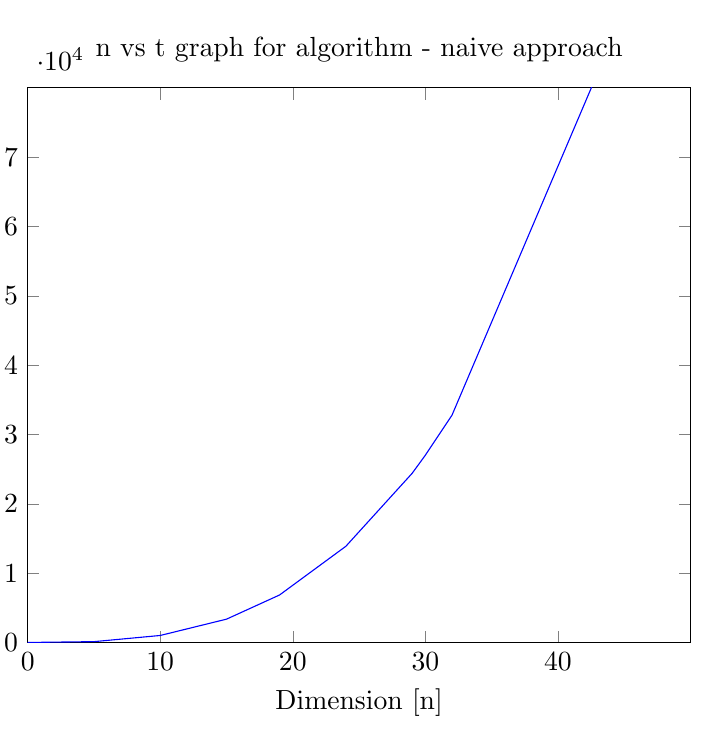
\begin{tikzpicture}[trim left=0cm]
\begin{axis}[
    title={n vs t graph for algorithm - naive approach},
    xlabel={Dimension [n]},
    ylabel={Time [t in ns]},
    xmin=0, xmax=50,
    ymin=0, ymax=80000,
    xtick={0,10,20,30,40},
    ytick={0,10000,20000,30000,40000,50000,60000,70000}
]
\addplot[
    color=blue,
    mark=dot,
    ]
    coordinates {
   (0,0)(5,120)(10,1010)(15,3365)(19,6851)(24,13874)(29,24399)(30,27023)(32,32758)(45,91168)
    };
    
  \end{axis}
  


\end{tikzpicture}



\begin{flushleft}

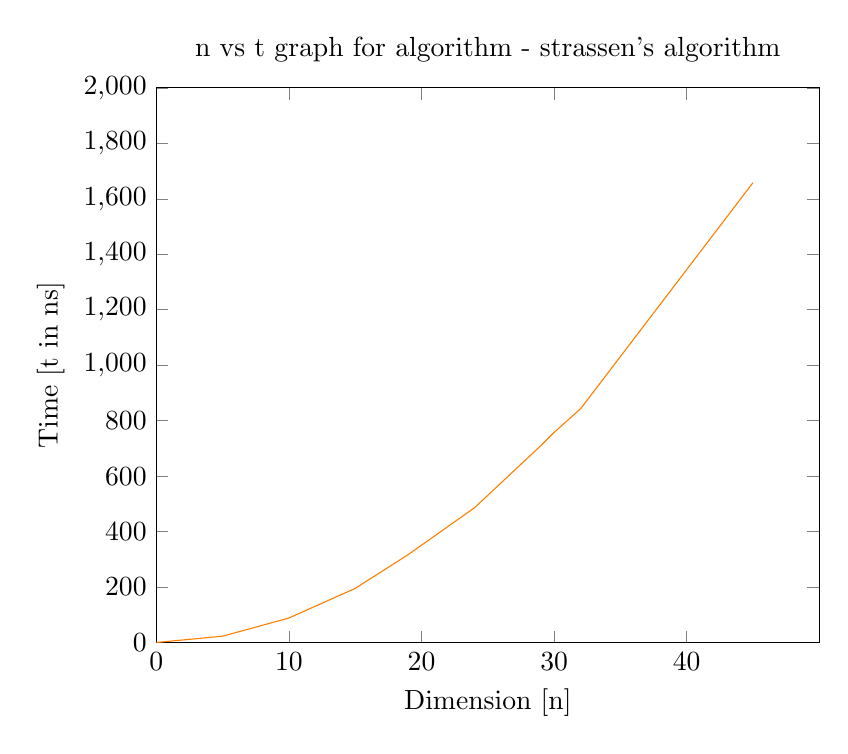
\begin{tikzpicture}
\begin{axis}[
    title={n vs t graph for algorithm - strassen's algorithm},
    xlabel={Dimension [n]},
    ylabel={Time [t in ns]},
    xmin=0, xmax=50,
    ymin=0, ymax=2000,
    xtick={0,10,20,30,40},
    ytick={0,200,400,600,800,1000,1200,1400,1600,1800,2000}
]
\addplot[
    color=orange,
    mark=dot,
    ]
    coordinates {
  (0,0)(5,22.81)(10,88.35)(15,195.12)(19,317.05)(24,486.02)(29,709.93)(30,757.64)(32,842.93)(45,1658.07)
    };
    
  \end{axis}
  


\end{tikzpicture}
\end{flushleft}


\section{CONCLUSION\\}
For matrix with higher dimension, Strassen's method to compute multiplication of matrices is significantly faster than naive method.\\

\section{Reference}
\begin{enumerate}

    \item \url{https://www.cs.cmu.edu/~15451-f19/LectureNotes/lec01-strassen.pdf}
        \item \url{https://en.wikipedia.org/wiki/Strassen\_algorithm}
\end{enumerate}



\end{document}


